% Copyright 2022 the authors

% To-Do list:
% -----------
% - What are our GOALS!!?
%   -- one option: this formulation can express all equivariant differential operators discretized to a cubical d-torus. 
%   -- another option: can we produce a characterization of all equivariant functions (maybe based on invariants or these filters) that don't require the use of non-linearities.
%   -- another option: emulate cosmological simulations.
% - change N to N^3 in the appropriate locations; already done??
% - Understand what functions can and cannot be expressed on this model 
% - Extend it to non-linear maps (eg, by multiplications and contractions)
% - Should we be representing images in fourier space? Ask Leslie!
% - Understand the literature
%   -- Discretized vector calculus and differential geometry.
%   -- Group-equivariant CNNs; what's been done?
%   -- Understand how this formulation compares with steerable CNNs
%   -- What is known about what functions CNNs can represent? all linear translation equivariant functions can be written as convvolutions if the filters are as large as the image (simple observation)
% what about non-linear? is there a polynomial basis here? 
%  -- Define "local" functions, is there a characterization of functions that can be written as convolutions with small filters?
% - There is a one-indexing and zero-indexing issue. Should we be consistent?
% - Some definitions begin with "given" some with "let". Should we try to be more consistent?

% -- if the size of the filter is large enough, are we universal???? or can we express all polynomial functions? is there a version of Stone-Weierstrass for this?
% --- add the identity and levi civita in the possible output tensors
% --- define reordering of the indices
% --- we don't need to be in the torus and we don't need to be square (or cubical)
% --- generalize convolution to rectangular non-toroidal images


%-- is it the same to do convolutions + products + convolutions + products 

%-- a counting argument may tell us that all the linear functions that are equivariant  (Molien's formula)

%-- BEN: compute Molien's formula for this (translations semidirect D_4) action
% 1/|G|\sum_{g\in G} det(I-\phi(g)t)^{-1}

% write the levi civita contraction
% write the procedure of which we make all linear functions from k tensor images to k' tensor images of the same size. 
% do we include a pooling move?

% how do we enumerate all tensor functions

% 1, 6, 22, 49, 87 d=3, n=1,3,7,9 (11N^2-24N+21)/8

\documentclass{article}
\usepackage[utf8]{inputenc}
\usepackage[letterpaper]{geometry} % because Overleaf is weird.
\PassOptionsToPackage{hyphens}{url}
\usepackage[hidelinks]{hyperref}
\usepackage{graphicx}
\usepackage{amsfonts}
\usepackage{amsmath}
\usepackage{amsthm}

% stuff for framing figures
\usepackage[framemethod=tikz]{mdframed}
\usetikzlibrary{shadows}
\definecolor{captiongray}{HTML}{555555}
\mdfsetup{%
  innertopmargin=2ex,
  innerbottommargin=1.8ex,
  linecolor=captiongray,
  linewidth=0.5pt,
  roundcorner=5pt,
  shadow=true,
  shadowcolor=black!05,
  shadowsize=4pt
}

% theorem, definition and so on
\theoremstyle{plain}
\newtheorem{definition}{Definition}
\newtheorem{conjecture}{Conjecture}
\newtheorem{theorem}{Theorem}

% math macros
% HOGG SAY: I DON'T KNOW HOW TO USE AMSMATH \choose AND I'M ON A PLANE. FEEL FREE TO FIX THIS.
\renewcommand{\choose}[2]{\begin{pmatrix}{#1}\\{#2}\end{pmatrix}}

% text macros
\newcommand{\sectionname}{Section}
\newcommand{\secref}[1]{\sectionname~\ref{#1}}
\newcommand{\figref}[1]{\figurename~\ref{#1}}

% typesetting adjustments
\makeatletter
\renewcommand\section{\@startsection {section}{1}{\z@}%
  {-3.25ex \@plus -1ex \@minus -.2ex}%
  {1.5ex \@plus .2ex}%
  {\raggedright\normalfont\large\bfseries}}% key thing is: \raggedright!
\makeatother
\setlength{\textwidth}{5.00in}
\setlength{\oddsidemargin}{3.25in}
\addtolength{\oddsidemargin}{-0.5\textwidth}
\setlength{\textheight}{9.40in}
\setlength{\topmargin}{-0.50in}
\setlength{\footskip}{0.25in}
\pagestyle{myheadings}
\markboth{foo}{Hogg, Blum-Smith, \& Villar / Geometric filters for geometric images}
\newcommand{\figurerule}{\rule[1ex]{\textwidth}{0.2pt}}
\linespread{1.08}
\frenchspacing\sloppy\sloppypar\raggedbottom

\title{\bfseries%
Convolution-based nonlinear functions on tensor fields and tensor images}
\author{David W. Hogg, Ben Blum-Smith, and Soledad Villar}
\date{}

\begin{document}

\maketitle\thispagestyle{empty}

\paragraph{Abstract:}
Convolutional neural networks are the main tools for machine learning with images at the present day.
These methods effectively assume that the input images are scalar images (an intensity or brightness in each pixel, possibly in three or more channels), and they enforce a kind of locality and translation-equivariance.
In natural-science domains, image-like data sets can have a vector (velocity, say), or tensor (polarization, say), or pseudovector (magnetic field, say), or any combination in each pixel.
We provide a construction for general convolution-based functions of images or lattices
containing scalars, vectors, and tensors, producing scalar, vector, and tensor outputs.
Our formulation, which combines a geometric generalization of convolution with products, tensor index contractions, contractions with Levi-Civita symbols, and tensor index permutations, can universally approximate any suitably local analytic scalar, vector, or tensor functions on scalar, vector, or tensor images.
The framework permits, with a very simple adjustment, restriction to function spaces that are exactly equivariant to translations, discrete rotations, and reflections, but the framework will be useful even in contexts in which the functions are not expected to be equivariant.

\section{Introduction}

Contemporary natural science teems with data sets that are images or lattices or grids of geometric objects.
These might be observations of intensities (scalars), magnetic fields (pseudovectors), or polarizations (2-tensors) on a surface or in a volume.
Or they might be the inputs or outputs of a simulation, in which the initial conditions or fields are specified on a regular grid.
Any lattice or grid of vectors or tensors can be seen as a generalization of the concept of an image, in which the intensity in each pixel is replaced with a geometric object (scalar, vector, pseudovector, tensor) in each pixel.
These objects are \emph{geometric} in the sense that they are defined in terms of their transformation properties under geometric operators such as rotation, translation, and reflection.
Thus there is a need for machine learning methods designed for \emph{geometric images}---lattices or grids of scalars, vectors, and tensors.
There are already countless applications of machine learning in contexts in which the input data are geometric images, including examples in essentially all natural-science disciplines (for example, CITE).

%For a concrete example close to one of our hearts (DWH's), contemporary cosmological n-body simulations comprise the most computationally expensive part of most contemporary cosmological projects, missions, and experiments (CITE THINGS).
%For this reason, accurate, fast emulators might be of enormous economic and scientific value.
%There are now quite a few successful projects implementing such emulators (CITE THINGS).
%Importantly, the initial conditions for these simulations are tiny displacements (vectors) and velocities (vectors) relative to a cubical lattice on a 3-torus.
%That is, the initial conditions can be described as a 3-dimensional image of vectors on a regular grid.
%For another concrete example, astronomical imaging data taken of the interstellar medium can be represented as rectangular lattices of measurements of temperature (scalar), optical depth (scalar), and induced polarization of starlight (a 2-tensor).
%Here the data can be described as a 2-dimensional image of scalars and tensors on a regular grid.

At the present day, the go-to tools for machine learning with images are convolutional neural networks (CNNs; CITE) and their many descendents (for example, CITE).
These methods are designed to work on one- or few-channel images in which, at the bottom (early) layers of the network, the operations involve image convolutions with learned filters followed by the application of pointwise nonlinearities.
In typical contexts, the channels of multi-channel input images will be something like the red, green, and blue (or cyan, magenta, yellow, and black) channels of a color image; these can be combined arbitrarily in the layers of the CNN.
When these CNN-based tools are applied to lattices of vectors (say), typically the components of the vectors are treated just as channels of the input image (for an example, see CITE) and then everything proceeds as with multi-channel color images.
This is not good!

Actually, it \emph{is} good: There are many successful projects that have repurposed CNNs in this way to work on geometric images.
But there are even better choices.
Here we propose a set of tools that generalize the concept of convolution to apply to geometric images such that the outputs of the convolutions are also geometric images, obeying the same geometric transformation rules as the inputs.

The fundamental observation inspiring this work is that when the components of vectors and tensors are acted on with arbitrary functions, the geometric structure of these objects is destroyed.
There are strict rules, dating back to the invention of differential geometry (CITE RICCI++), about how geometric objects can be combined to produce new geometric objects, consistent with coordinate freedom and transformation rules.
In previous work (CITE VILLAR++, YAO++) we have capitalized on these geometric rules to develop modified machine-learning methods that are restricted to exactly obey group-theoretic equivariances in physics contexts.
Here we use these rules to create a comprehensive set of tools that are universally approximating for functions that take geometric images as input and produce geometric labels (or geometric-image labels) as output.

We are motivated in this work to help solve problems in the natural sciences, where geometric images abound.
However, we conjecture that these tools are probably very useful even for standard machine-learning image-recognition and image-regression tasks.
After all, even standard images are measurements of intensity (a scalar) at a regular grid of points on a two-dimensional surface.
If the labels we seek are also scalars, it will behoove us to obey the rules of geometry.

These rules are roughly as follows:
A $k$-tensor object (tensor of order $k$) in $d$ dimensions has $k$ indices, each of which can take a value from 1 to $d$; that is, the $k$-tensor is an element of $(\mathbb R^d)^{\otimes k}$.
It can be contracted to a $(k-2)$-tensor object by identifying a pair of indices and summing over them.
A $k$-tensor and a $k'$-tensor can be multiplied (outer product) to make a $(k+k')$-tensor object, and then contractions can bring down the order.
$1$-tensor objects are called vectors and $0$-tensor objects are called scalars.
There are also odd-parity versions of all these (pseudovectors, pseudoscalars, and pseudotensors), and parity-changing contractions using the Levi-Civita symbol, so in what follows we will define $k$-$p$-tensors that have $k$ indices and a parity $p\in [0, 1]$.
Two objects can only be added or subtracted if they have the same order $k$ and parity $p$.
This will all be made precise below.
But in short, these rules define objects that can be given transformation rules under rotation and reflection such that functions made of these operations are coordinate free, or equivariant to any change of coordinate system (including curvilinear coordinate transformations).

The symmetries that suggest these rules are continuous symmetries.
But of course images are usually---and for our purposes---discrete grids of values.
This suggests that in addition to the continuous symmetries respected by the tensor objects in the image pixels there will be discrete symmetries for each geometric image taken as a whole.
We will define these discrete symmetry groups and use them to define a useful kind of group equivariance for functions of geometric images.
This equivariance, it turns out, is very easy to enforce, even for nonlinear functions of geometric images, provided that we compose our nonlinear functions from simple geometric operations, including our geometric generalization of convolution.
When we enforce this equivariance, the convolution filters that appear look very much like the differential operators that appear in discretizations of vector calculus, which is perhaps not surprising.

\paragraph{Related work:}

\paragraph{Our contribution:}

\section{Geometric objects and geometric images}\label{sec:geometric}

In this \sectionname{} we define the geometric objects and geometric images that we use to generalize classical images in scientific contexts.
The main point is that the channels of geometric images---which will be like the components of vectors and tensors---are not independent.
There is an underlying action by the orthogonal group that rules what are the allowed objects and transformations in this space.

We first fix $d$, the dimension of the space (typically 2 or 3 but it could be arbitrary). The geometric objects are vectors and tensors. 
The orthogonal group $O(d)$ can act on $v \in \mathbb R^d$ in the following ways:
\begin{align} \label{eq.action}
    g\cdot v = \det(M(g))^p M(g) v 
\end{align}
where $g\in O(d)$, $M(g)\in \mathbb R^{d\times d}$ is the standard matrix representation of $g$, and $p\in\{0,1\}$ is the parity of the action. If $p=0$ we obtain the standard $O(d)$ action on $\mathbb R^d$ \emph{vectors}. If $p=1$ we obtain what in physics is commonly known as the action of $O(d)$ on \emph{pseudovectors}. In this context the objects are defined by the actions that they carry.

\begin{definition}[$k$-$p$-tensors] \label{def.tensors}
We say that $v\in \mathbb R^d$ is a 1-$p$-tensor if $O(d)$ acts on $v$ via the action \eqref{eq.action}. 
If $v_i$ is a 1-$p_i$-tensor then $T:=v_{1}\otimes\ldots \otimes v_k$ is a rank-1 $k$-$p$-tensor, where $p=\sum_{i=1}^k p_i \mod 2$ and the action of $O(d)$ is defined as
\begin{align}
    g\cdot (v_{1}\otimes\ldots \otimes v_k) = (g\cdot v_1)\otimes \ldots \otimes (g\cdot v_k)
\end{align}
Higher rank $k$-$p$-tensors are defined as linear combinations of rank-1  $k$-$p$-tensors where the action of $O(d)$ is extended linearly.
\end{definition}
Typically we would make the parity $p$ be a bit (either 0 for even parity or 1 for odd parity) but in principle it can be any integer.

We note that in physics the 1-0-tensors are known as \emph{vectors}, the 1-1-tensors are known as \emph{pseudovectors}, the 0-0-tensors are known as \emph{scalars}, 0-1-tensors are known as \emph{pseudoscalars}, the $k$-1-tensors with $k\geq 2$ are known as \emph{pseudotensors}, and finally the $k$-0-tensors with $k\geq 2$ are the things that are commonly known as \emph{tensors}.

\begin{definition}[summation notation]
In this notation, tensor products are written in component form, and repeated indices are summed over.
In this notation, the product of two 2-tensors (represented as two $d\times d$ matrices $A$ and $B$) is written as
\begin{equation}
    [A\, B]_{i,j} = [A]_{i,k}\,[B]_{k,j} ~,
\end{equation}
where $[A]_{i,k}$ (for example) is the $i,k$ element of matrix $A$, the repeated index $k$ is implicitly summed over the integers from 1 to $d$.
This notation works for tensor expressions of any order, provided that every index appears either exactly once (so it isn't summed over; in the above expression $i, j$ appear exactly once) or exactly twice (so it is summed over; in the above expression $k$ appears exactly twice). 
\end{definition}

One consequence of the above definitions is that 
$T\in (\mathbb R^d)^{\otimes k}$ is a $k$-$p$-tensor if and only if (in summation notation)
\begin{align}
    [g\cdot T]_{i_1,\ldots, i_k} = \det(M(g))^p\, [T]_{j_1,\ldots,j_k}\,[M(g)]_{i_1,j_1}\cdots[M(g)]_{i_k,j_k}
\end{align} for all $g\in O(d)$, where $[T]_{i_1, \ldots ,i_k} \in \mathbb R$ is a component of $T$, $[M(g)]_{i,j}\in\mathbb R$ is the $i,j$ element of the matrix representation of $g$, and all the $i_m$ and $j_m$ are indices in the range $1,\ldots,d$.
For example, a 2-0-tensor is defined by its transformation property
$[g\cdot T]_{i,j} = [T]_{k,\ell}\,[M(g)]_{k,i}\,[M(g)]_{\ell,j}$,
which, in normal matrix notation, is written as
$g\cdot T = M(g)\,T\,M(g)^\top$.

We consider an image $A$ in with $N$ equally spaced pixels in each dimension ($N^d$ pixels total). Each pixel contains a $k$-$p$-tensor ($k$ and $p$ are the same for each pixel). Sometimes we will consider the image to be in a $d$-torus. 
Let $\mathcal T_{d,k,p}$ the set of $k$-$p$-tensors in $\mathbb R^d$. We define the geometric images as follows.
\begin{definition}[geometric image]
A geometric image is a function $A:[N]^d \to \mathcal T_{d,k,p}$, where $[N]=\{0,1,\ldots, N-1\}$. We will also consider $k$-tensor images on the $d$-torus, where $[N]^d$ is given the algebraic structure of $(\mathbb Z / N\mathbb Z)^d$.
\end{definition}

\section{Generalized convolutions on geometric images}\label{sec:convolution}

In this \sectionname{} we generalize the notion of convolution to take geometric images as inputs and return geometric images as outputs.
The idea is that the (presumably large) geometric image (containing $k$-$p$-tensors) is convolved with a (presumably small) geometric filter (also a geometric image, but containing $k'$-$p'$-tensors) to produce an output image that contains $(k+k')$-$(p+p')$-tensors, where each pixel is a sum of outer products.
These outer products can be contracted down to lower-$k$ tensors using Kronecker or Levi-Civita contractions.

\begin{definition}[outer products of tensors]
If $a$ is a $k$-$p$-tensor and $b$ is a $k'$-$p'$-tensor, then the outer product $a\otimes b$ is a $(k+k')$-$(p+p')$-tensor with $[a\otimes b]_{i_1,\ldots,i_{k+k'}} = [a]_{i_1,\ldots,i_k}\,[b]_{i_{k+1},\ldots,i_{k+k'}}$.
\end{definition}

SOLE: If the next definition is going to use ``the torus'' then we should say a few words about that up-front, or above in the image definition.

\begin{definition}[geometric convolution]
Let $A$ be a $k$-$p$-tensor image on the $d$-torus with side length $N$.
Let $C$ be a $k'$-$p'$-tensor image (filter) on $[-m, m]^d$ where $2m+1<N$.
The geometric convolution $A\ast C$ is a $(k+k')$-$(p+p')$-tensor image such that
\begin{equation}
    (A\ast C)(\bar\i) = \sum_{\bar a\in[-m, m]^d} A(\bar\i - \bar a)\otimes C(\bar a) ~,
\end{equation}
where $\bar\i - \bar a$ is the translation of $\bar\i$ by $\bar a$ on the $d$-torus pixel grid $(\mathbb Z / N\mathbb Z)^d$.
\end{definition}
This definition is on the torus. If you are not on the torus, just pad the image out with zero tensors of the corresponding order and parity. 

Convolutions can be followed by Kronecker contractions, Levi-Civita contractions and index permutations.
The Kronecker delta ($\delta_{ij}$) is the object with two indices $ij$ such that it has the value $+1$ when the two indices have the same value ($i=j$), and $0$ otherwise.
Below we define the contraction of a $k$-$p$-tensor (with $k\geq 2$) with one application of the Kronecker delta, which returns a $(k-2)$-$p$-tensor.
The Levi-Civita symbol in $d\geq 2$ spatial dimensions is the object with $d$ indices (where $d$ is the spatial dimension) such that if the $d$ indices are not repeated and in an even-permutation order the value is $+1$ and if the $d$ indices are not repeated and in an odd-permutation order the value is $-1$, and it has the value $0$ in all other cases.
We define the contraction of a $k$-$p$-tensor (with $k\geq (d-1)$) with one application of the Levi-Civita symbol, which returns a $(k-d+2)$-$(p+1)$-tensor, because the contraction sums over $d$ pairs of indices, and it changes the parity from even to odd or odd to even.
For one example of these contractions, the 2-tensor formed by the outer product of 1-tensors $a$ and $b$ can be contracted with the Kronecker delta to give the standard dot product $a^\top b = [a]_i\,[b]_j\,\delta_{ij}$, which is a 0-tensor or scalar.
For another example, the same 2-tensor can (in $d=3$ dimensions) be contracted with the Levi-Civita symbol to give the standard cross product
$[a\times b]_k = [a]_i\,[b]_j\,\epsilon_{ijk}$, which is a pseudovector.

\begin{definition}[Kronecker contractions of tensors and geometric images]
Let $a$ be a $k$-$p$-tensor in $\mathbb R^d$ with $k\geq 2$ such that $[a]_{i_1,\ldots i_k}\in \mathbb R$ for all $i_s = 1,\ldots, d$, and $s=1,\ldots, k$. We define the $(\alpha,\beta)$ Kronecker contraction of $a$ to be the $k-2$ tensor resulting from summing jointly over the indices $i_\alpha$ and $i_\beta$ where $\alpha < \beta \in\{1,\ldots, k\}$. In Einstein summation notation it would be $a_{i_1, \ldots, x, \ldots , x, \ldots, i_k}$ where the $x$s are placed in the positions $\alpha$ and $\beta$:
\begin{equation}
[a^{(\alpha,\beta)}]_{i_1, \ldots, i_k \backslash i_\alpha,i_\beta} := \sum_{i_\alpha=1}^d \sum_{i_\beta=1}^d [a]_{i_1, \ldots, i_\alpha,\ldots,i_\beta,\ldots, i_k}\,\delta_{i_\alpha, i_\beta}
\end{equation}
When Kronecker contraction is applied to a geometric image, the contraction is applied to every $k$-$p$-tensor in the image identically.
\end{definition}
There are $\choose{k}{2}$ different index choices for this contraction, corresponding to all the possible index pairs among $k$ original indices.

\begin{definition}[Levi-Civita contractions of tensors and geometric images]
Let $a$ be a $k$-$p$-tensor in $\mathbb R^d$ with $k\geq d-1$ such that $[a]_{i_1,\ldots i_k}\in \mathbb R$ for all $i_s = 1,\ldots, d$, and $s=1,\ldots, k$. We define the Levi-Civita contraction of $a$ to be the $(k-d+2)$-$(p+1)$-tensor resulting from taking the outer product of 
$a$ with the $d$-index Levi-Civita symbol $\epsilon_{i_1,i_2,\ldots,i_d}$ and then performing $d-1$ Kronecker contractions in which the first index is chosen from the (remaining) indices of $a$ and the second index is chosen from the (remaining) indices of the Levi-Civita symbol.
When a Levi-Civita contraction is applied to a geometric image, the contraction is applied to every $k$-$p$-tensor in the image identically.
\end{definition}
There are $(d-1)!\,\choose{k}{d-1}$ different index choices for the Levi-Civita contraction of a $k$-$p$-tensor.
These choices correspond to the choices for an ordered list of $d-1$ indices chosen from among $k$ index choices.

\begin{definition}[permutations of tensor indices]
Given a $k$-$p$-tensor $a$ and $\sigma\in S_k$ a permutation. We consider $a^\sigma$ the result of permuting the indices of $a$ according to $\sigma$:
\begin{equation}
    [a^\sigma]_{i_1, \ldots, i_k} := [a]_{\sigma^{-1}(i_1), \ldots, \sigma^{-1}(i_k)}
\end{equation}
When index permutation is applied to a geometric image, the permutation is applied to every $k$-$p$-tensor in the image identically.
\end{definition}

In addition to these contractions and index permutations that act pixel-wise in geometric images, it is possible to change the image size.
If $N$ is divisible by integer $f>1$, a geometric image of side length $N$ can be reduced in size to a geometric image of side length $N/f$ by the equivalent of convolution with a trivial $f\times f$ scalar filter (geometric filter of 0-0-tensors) operating with a stride of $f$.
Similarly a geometric image of side length $N$ can be expanded in size to a side length $f\,N$ by application of an interpolation operator with stride $1/f$.
\begin{definition}[pooling and un-pooling]
foo and bar.
\end{definition}

Now imagine that we want to find \emph{all} linear equivariant functions that go from an input $k$-$p$-tensor image of side length $N$ to an output $k'$-$p'$-tensor image of side length $N'$ (where either $N$ is divisible by $N'$, or $N'$ is divisible by $N$).
Here are the linear operations (linear in the input image) that are permitted:
\begin{enumerate}
    \item Perform a convolution and index contraction. For this step there are two qualitatively different options:
        \begin{itemize}
            \item Choose an integer $\ell$ in the range $0\leq\ell\leq k$ such that $(k'-k+2\,\ell)>0$.
              Convolve the input $k$-tensor image with a $(k'-k+2\,\ell)$-tensor invariant filter of parity $p\,p'$.
              Contract the resulting $(k'+2\,\ell)$-tensor image (of parity $p'$) with the Kronecker delta $\ell$ times, always choosing at least one index from the indices of the input image.
              There are $$\frac{1}{\ell!}\,\prod_{i=1}^{\ell}\left[\choose{k'+2\,i}{2}-\choose{k'-k+2\,i}{2}\right]$$ possible choices for these $\ell$ Kronecker contractions.
            \item Choose an integer $\ell$ in the range $0\leq\ell\leq k-d+1$ such that $(k'-k+d-2+2\,\ell)>0$.
              Convolve the input $k$-tensor image with a $(k'-k+d-2+2\,\ell)$-tensor invariant filter of parity $-p\,p'$.
              Contract the resulting $(k'+d-2+2\,\ell)$-tensor image (of parity $-p'$) with the Levi--Civita symbol.
              There are $$(d-1)!\,\left[\choose{k'+d-2+2\,\ell}{d-1}-\choose{k'-k+d-2+2\,\ell}{d-1}\right]$$ choices for this Levi--Civita contraction.
              Then contract the resulting $(k'+2\,\ell)$-tensor image (of parity $p'$) with the Kronecker delta $\ell$ times, always choosing one index from the indices of either the input image or of the Levi--Civita symbol.
              There are $$\frac{1}{\ell!}\,\prod_{i=1}^{\ell}\left[\choose{k'+2\,i}{2}-\choose{k'-k+2\,i}{2}\right]$$ possible choices for these $\ell$ Kronecker contractions.
        \end{itemize}
    \item Perform (generally after the convolution and contraction) any index permutation you like (provided that $k'>1$).
      There are $k'!$ choices for the index permutation.
    \item Perform (generally after all the above) a pooling or unpooling step to get the image to side length $N'$.
\end{enumerate}
The objects obtained by this algorithm may not be linearly independent.

In principle there could also have been an \emph{eigenvalues} operator that is linear in the input and produces $d$ $0$-$p$-tensors.
But since any such operation can only reasonably be applied to $2$-$p$-tensors, and even for those, only Hermitian ones, we don't include this operation here.

\section{Higher-order functions of geometric images}\label{sec:nonlinear}

The convolution, contraction, index-permutation, and pooling operators above effectively span a large class of linear functions from geometric images to geometric images. Non-linear functions can be constructed as polynomials, or sums of products of linear function outputs.
Products here will be outer products (possibly followed by further geometric convolutions and contractions).

\begin{definition}[outer products of images]
Given a $k$-$p$-tensor image $A$ and a $k'$-$p'$-tensor image $B$, both of side length $N$, the outer product $A\otimes B$ of these images is a $(k+k')$-$(p+p')$-tensor image such that
\begin{equation}
    (A\otimes B)(\bar\i) = A(\bar\i)\otimes B(\bar\i) ~.
\end{equation}
That is, the outer products of geometric images are performed pixelwise.
\end{definition}

\begin{definition}[sums of images]
Given a $k$-$p$-tensor image $A$ and a $k$-$p$-tensor image $B$, both of side length $N$, the sum $A+B$ of these images is a $k$-$p$-tensor image such that
\begin{equation}
    (A+B)(\bar\i) = A(\bar\i)+B(\bar\i) ~.
\end{equation}
That is, the sums of geometric images are performed pixelwise.
\end{definition}

Now to construct all degree-2 monomials that produce a $k'$-$p'$-tensor image of side length $N'$ output from a $k$-$p$-tensor image of side length $N$ input, here are the rules:
\begin{enumerate}
    \item By the rules in \secref{sec:convolution}, construct any linear function that takes the input geometric image and outputs a geometric image of any order $k''$ and any parity $p''$ and any side length $N''$.
    \item By the rules in \secref{sec:convolution}, construct any other linear function that takes the input geometric image and outputs a geometric image of any order and any parity.
    There is no need for this second output image to be the same order or parity as the first, but it does have to have the same side length.
    \item Outer product these two images.
    \item By the rules in \secref{sec:convolution}, construct any linear function that takes this image outer product as input and produces a $k'$-$p'$-tensor image of side length $N'$ as output.
\end{enumerate}

We conjecture that these rules will generate all possible second-degree monomial functions of the input image (SOLE SUBJECT TO SOME CONDITIONS) that meet the output requirements. A polynomial function of degree 2 can be constructed by linear combinations of these second-degree monomial functions along with all the linear functions that also produce $k'$-$p'$-tensor images of side length $N'$ (plus perhaps constant images).
Higher-degree monomials and polynomials can be made out of products of lower-degree monomials, by generalization of the above.

SOLE: THIS PARAGRAPH OR THESE IDEAS GO ELSEWHERE, I THINK.
The geometric convolutions of \secref{sec:convolution} are local linear operators that take as input geometric images, and produce as output geometric images.
They are local in the sense that, at every pixel $\bar\i$ of the output image $(A\ast C)$, the convolution only makes use of the pixels of $A$ within a small neighborhood of of $\bar\i$.
Because tensors can be multiplied together using the outer product, and contracted according to the tensor contractions defined in \secref{sec:convolution}, it is possible, by multiplication, to construct a family of \emph{nonlinear} local geometric operators that take as input geometric images and produce as output geometric images.
This family of nonlinear local operators will be equivariant to the group $G_d$ when the linear local operators of which they are composed are equivariant.

\section{Equivariant functions of geometric images}\label{sec:equivariant}

Introduce the discrete group. Why discrete? SOLE: SEE TEXT BELOW FOR DEFINITIONS.

Define equivariance.

Prove translation invariance.

Prove things about invariant filters and equivariant linear functions.

\begin{definition}[Group $B_d$ of symmetries of a $d$-hypercube]
We denote by $B_d$ the group of rotation and reflection symmetries of the $d$-dimensional hypercube.
\end{definition}

Notes about the group $B_d$: In $d=2$ there are $8$ group elements, in $d=3$ there are $48$ group elements (and in $d=4$ there are 384). Because the groups $B_d$ are subgroups of $O(d)$, all determinants of the matrix representations of the group elements are either $+1$ or $-1$, and the matrix representation $M(g^{-1})$ of the inverse $g^{-1}$ of group element $g$ is the transpose of the matrix representation $M(g)$ of group element $g$.

\begin{definition}[Action of $B_d$ on $k$-$p$-tensors]
\begin{align}
g\cdot(v_1 \otimes \ldots \otimes v_k) &= \det(g)^p\,(g\cdot v_1)\otimes\ldots\otimes(g\cdot v_k)
\end{align}
And extend linearly
\end{definition}

This may seem familiar: The $k$-tensor and $k$-pseudotensor were defined by how they transform under the orthogonal group $O(d)$, and our group $B_d$ is a subgroup of the orthogonal group.

\begin{definition}[Action of $B_d$ on $k$-tensor images]
Given a $k$-tensor image $A$ on the $d$-torus, and a group element $g\in B_d$, the action $g\cdot A$ produces a $k$-tensor image on the $d$-torus such that
\begin{equation}
    (g\cdot A)(\bar\i) = g\cdot A({g^{-1}\cdot \bar\i}) ~.
\end{equation}
SOmeThiNg about how $g^{-1}\cdot\bar\i$ works here, possibly preceded or followed by proofs. Because of what follows, this has to be defined BOTH for the $N^d$ boxels in the $d$-torus and on the $(2\,m+1)^d$ boxels of the filter (image patch).
\end{definition}

It might be a bit surprising that the group element $g^{-1}$ appears in the definition of the action of the group on images.
One way to think about it is that the pixels in the output (rotated, say) image are ``looked up'' or ``read out'' from the pixels in the original (unrotated) image.
The pixel locations in the original image are found by going back, or inverting the transformation.

HOGG: Make a table and a figure showing all the group operators in $B_d$ with $d=2$.

\begin{definition}[The group $G_d$, and its action on $k$-tensor images]
THIS NEEDS TO BE WRITTEN: $G_d$ is the group generated by the elements of $B_d$ and the discrete translations on the $N^d$-pixel lattice on the $d$-torus.
\end{definition}

HOGG: Comment on the fact that $G_d$ is a subgroup of the Euclidean group, but that we care about the Euclidean group because we are imagining that the discrete images are images of a continuous world!!

\begin{definition}[Equivariant convolution]
We say that a convolution filter $C$ produces convolutions that are equivariant with respect to the group $G_d$ if for any $k$-tensor image $A$ on the $d$-torus, and any group element $g\in G_d$, we have
\begin{equation}
    g\cdot (A\ast C) = (g\cdot A)\ast C ~,
\end{equation}
where the group actions are defined above.
\end{definition}

The intuition here is that the filter $C$ represents some physical law, and the image $A$ represents the initial conditions or state of the physical system on which the law is acting.
The physical law (represented by $C$) is invariant to translations, rotations, and parity, while the \emph{output} of the physical law (represented by $A\ast C$) is \emph{equivariant} to translations, rotations, and parity acting on the state $A$.

The following theorem generalizes the Cohen and Welling paper:

\begin{theorem}
A $k'$-tensor (or $k'$-pseudotensor) convolution filter $C$ produces convolutions that are equivariant with respect to the big group $G_d$ if $C$ is invariant under the small group $B_d$.
\end{theorem}

\begin{proof}
By Definition \ref{} we have
\begin{eqnarray}
(g\cdot (A* C) )(\bar \i) &=& g\cdot( (A*C)(g^{-1} \cdot \bar \i)) \\
&=& g \cdot \left (\sum_{a\in [-m,m]^d} A(g^{-1}\cdot \bar \i - a) \otimes C(a)\right)\\
&=& \sum_{a\in [-m,m]^d} g \cdot A(g^{-1} \cdot \bar \i -a ) \otimes g \cdot C(a).
\end{eqnarray}
By Definition \ref{} we have
\begin{eqnarray}
((g\cdot A)* C) (\bar \i) &=& \sum_{a\in [-m,m]^d} g\cdot A(g^{-1} \cdot (\bar \i - a) ) C(a) \\
&=& \sum_{a'\in [-m,m]^d} g \cdot A(g^{-1}\cdot \bar \i -a') \otimes C(g\cdot a'),
\end{eqnarray}
where $a'=g\cdot a$. Therefore the convolution is equivariant if $g\cdot C(g^{-1} \cdot a') = C(a')$ for all $g\in B_d$ and all $a' \in [-m,m]^d$. 
\end{proof}

In practice, a complete set of invariant $k'$-$p'$-tensor filters (filters $C$ such that $g\cdot C(g^{-1} \cdot a') = C(a')$) can be found by group averaging.
This works by building any set of linearly independent $k'$-$p'$-tensor filters (randomly or systematically), and then building, for each of these linearly independent filters $C$, a group-averaged filter $\bar{C}$ by
\begin{equation}
    \bar{C}(a') = \frac{1}{|B_d|}\,\sum_{g\in B_d} g\cdot C(g^{-1}\cdot a') ~,
\end{equation}
where $|B_d|$ is the number of group elements (8 for $d=2$ and 27 for $d=3$).
In detail we took a systematic (not random) approach that initialized the averaging with a set of independent $k'$-$p'$-tensor convolution filters that span the space of all possible geometric convolution filters at side length $M$ ($M=2\,m+1$) and dimension $d$.
There are $M^d\,d^{k'}$ independent filters in this initial set.
The averaged filters are then reduced to an ``eigen-set'' of orthogonal, non-zero filters by the singular-value decomposition.
The singular-value decomposition reduces the number of filters dramatically.
The outputs of the singular-value decomposition can be normalized however seems appropriate.
In detail we normalized to get unit tensor norms in the non-zero pixels.
The results of these operations are shown for $d=2$ and $m\in[1, 2]$ in \figref{fig:filters23} and \figref{fig:filters25}.
HOGG: Give a table saying how many filters there are for each tuple of $(d,m,k',p')$.
HOGG: Perhaps remind the reader that the code is available.
\begin{figure}[tp]
  \begin{mdframed}
  \color{captiongray}
  \begin{center}
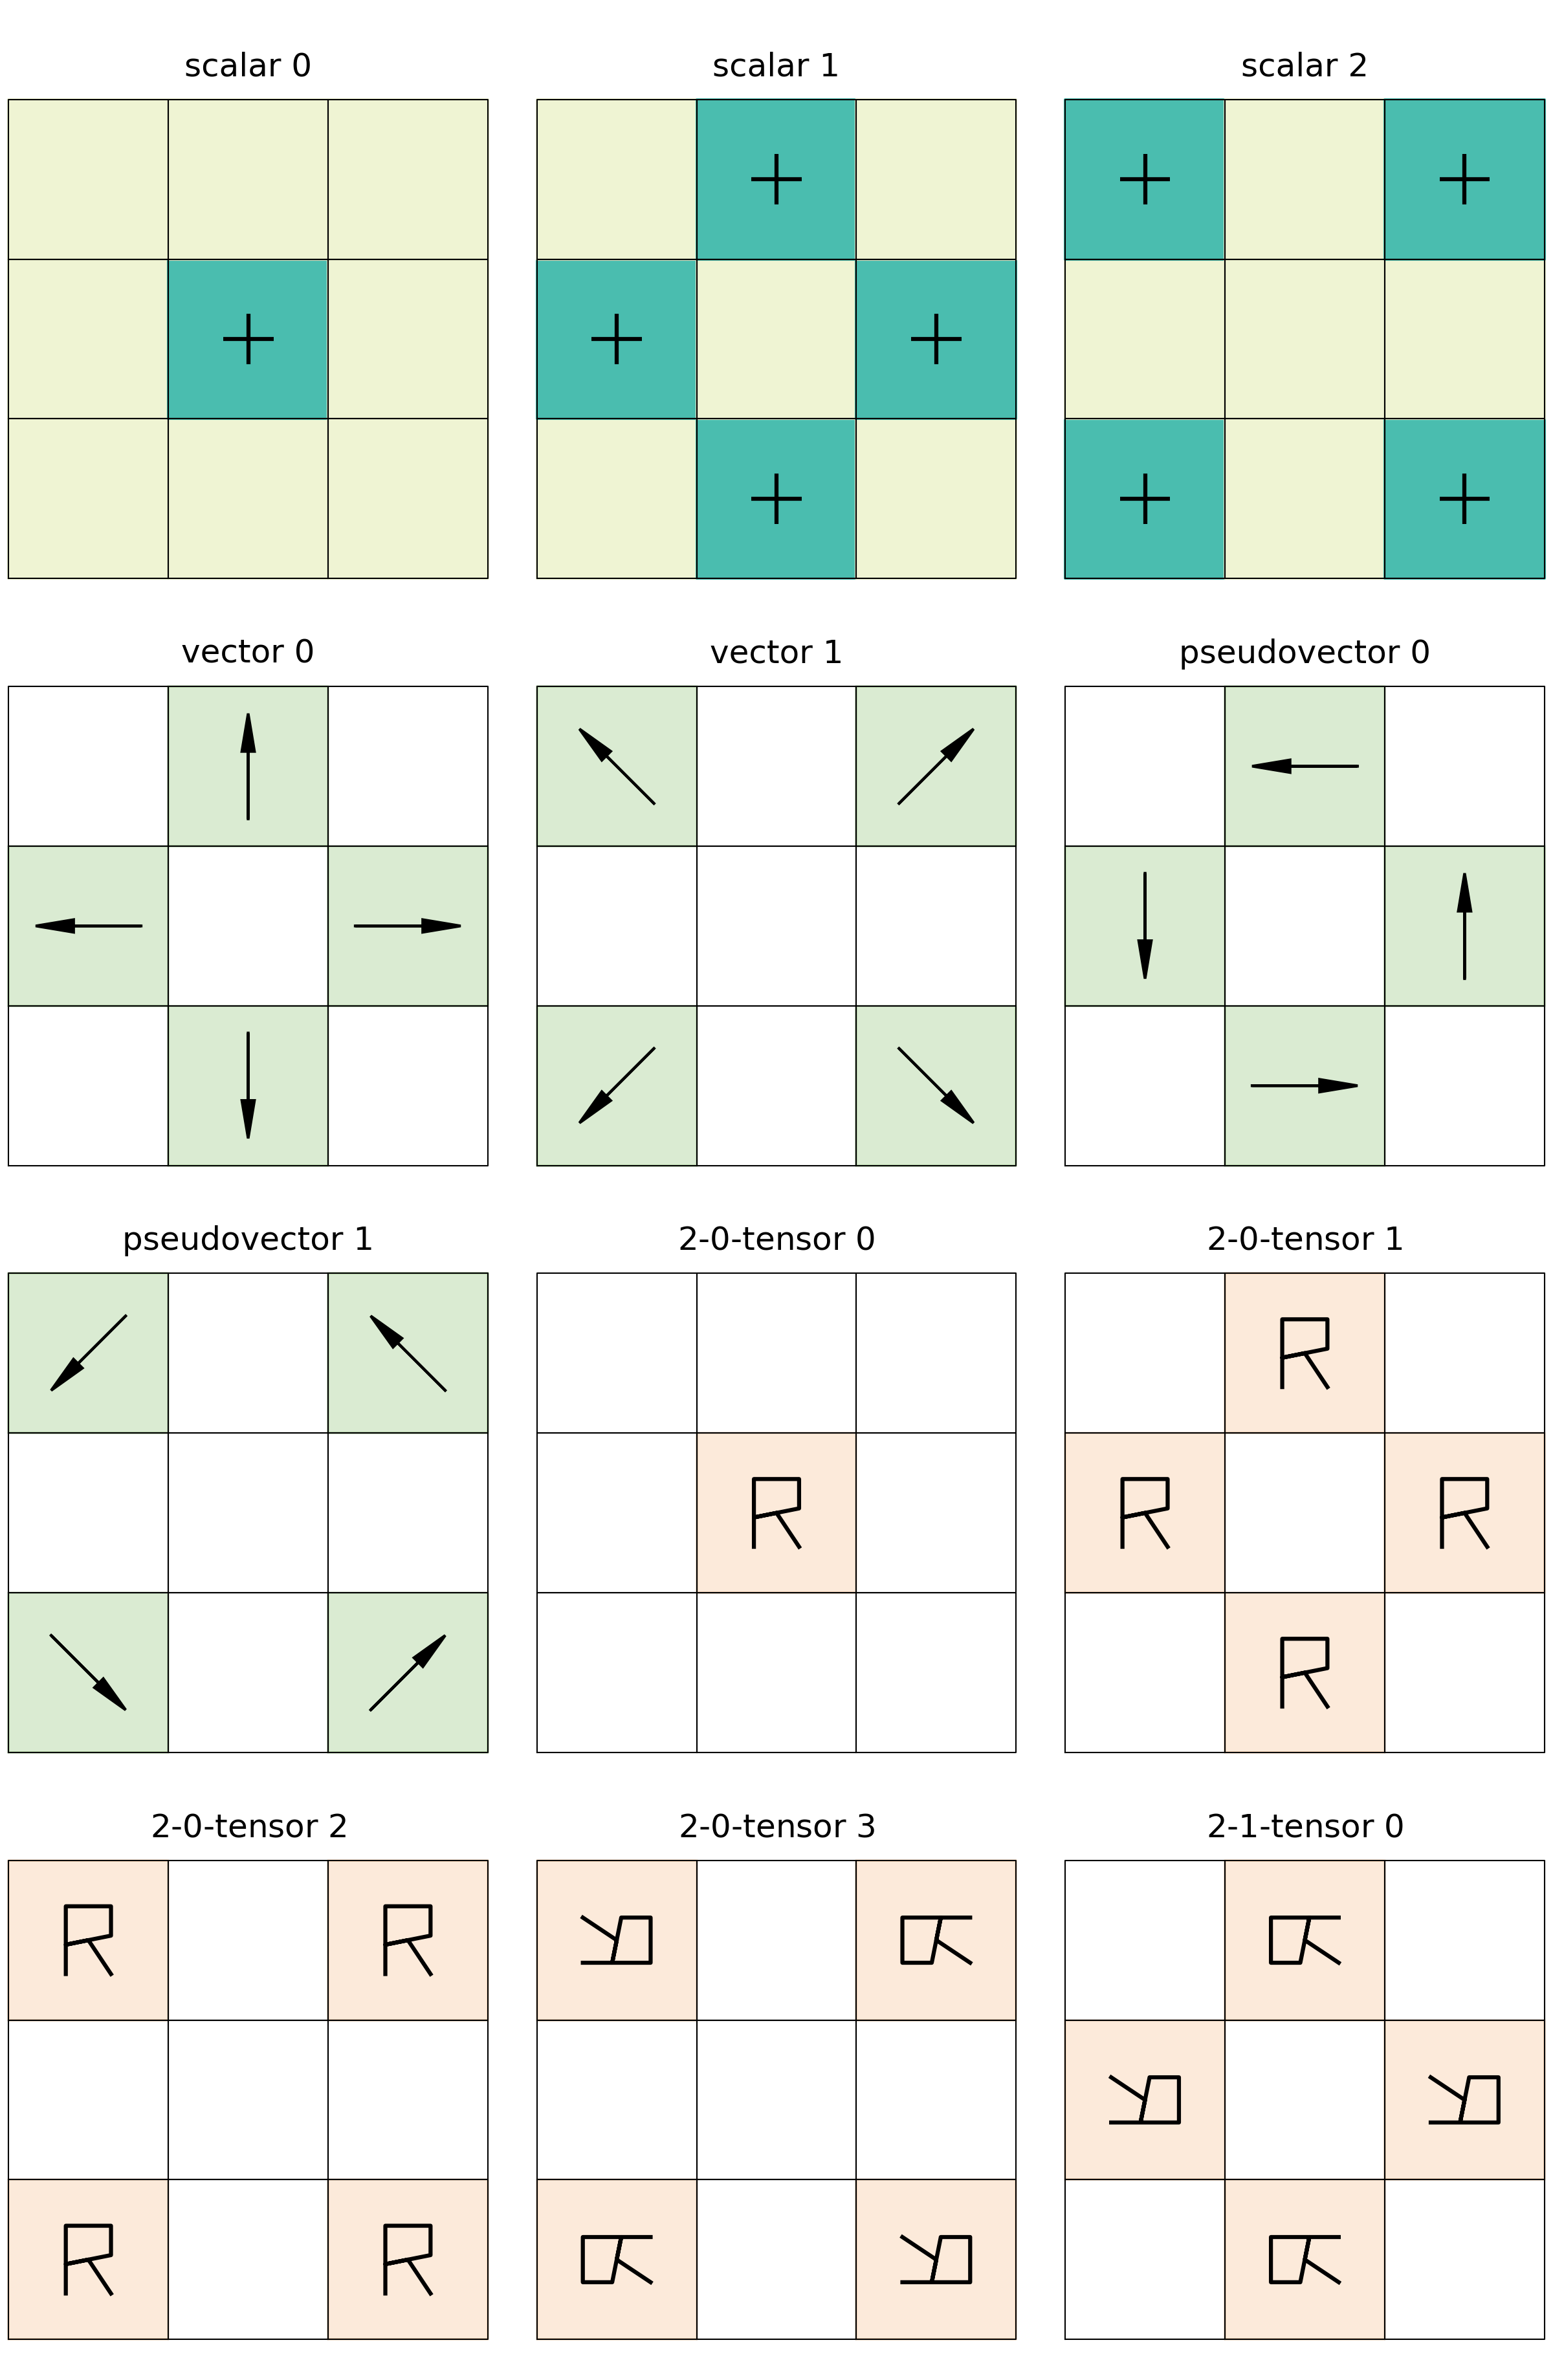
\includegraphics[width=\textwidth]{notebooks/filter_2_3.png}
  \end{center}
\caption{All the filters for $d=2$, $m=1$ ($M=3$).
Notes: Scalars and pseudo-scalars are shown with signed colors; where there is no symbol in the box the value is zero. The $2$-$p'$-tensor filters are shown via the action of the tensor on an image of a letter ``R''; the transformation properties of the $2$-$p'$-filters are such that these filters may not look obviously invariant to rotations, but they are.
There are no invariant pseudoscalar ($0$-$1$-tensor) filters available at $(d,m) = (2,1)$.
Three of the $2$-$0$-tensors are duplicates of the $0$-$0$-tensor (scalar) filters but multiplied by the identity tensor; there is only one non-trivial invariant $2$-$0$-tensor filter.
We don't show the $k'$-$p'$-filters at $k'>2$ because we don't know how to visualize them (even the $k'=2$ case is sketchy).\label{fig:filters23}}
  \end{mdframed}
\end{figure}
\begin{figure}[tp]
  \begin{mdframed}
  \color{captiongray}
  \begin{center}
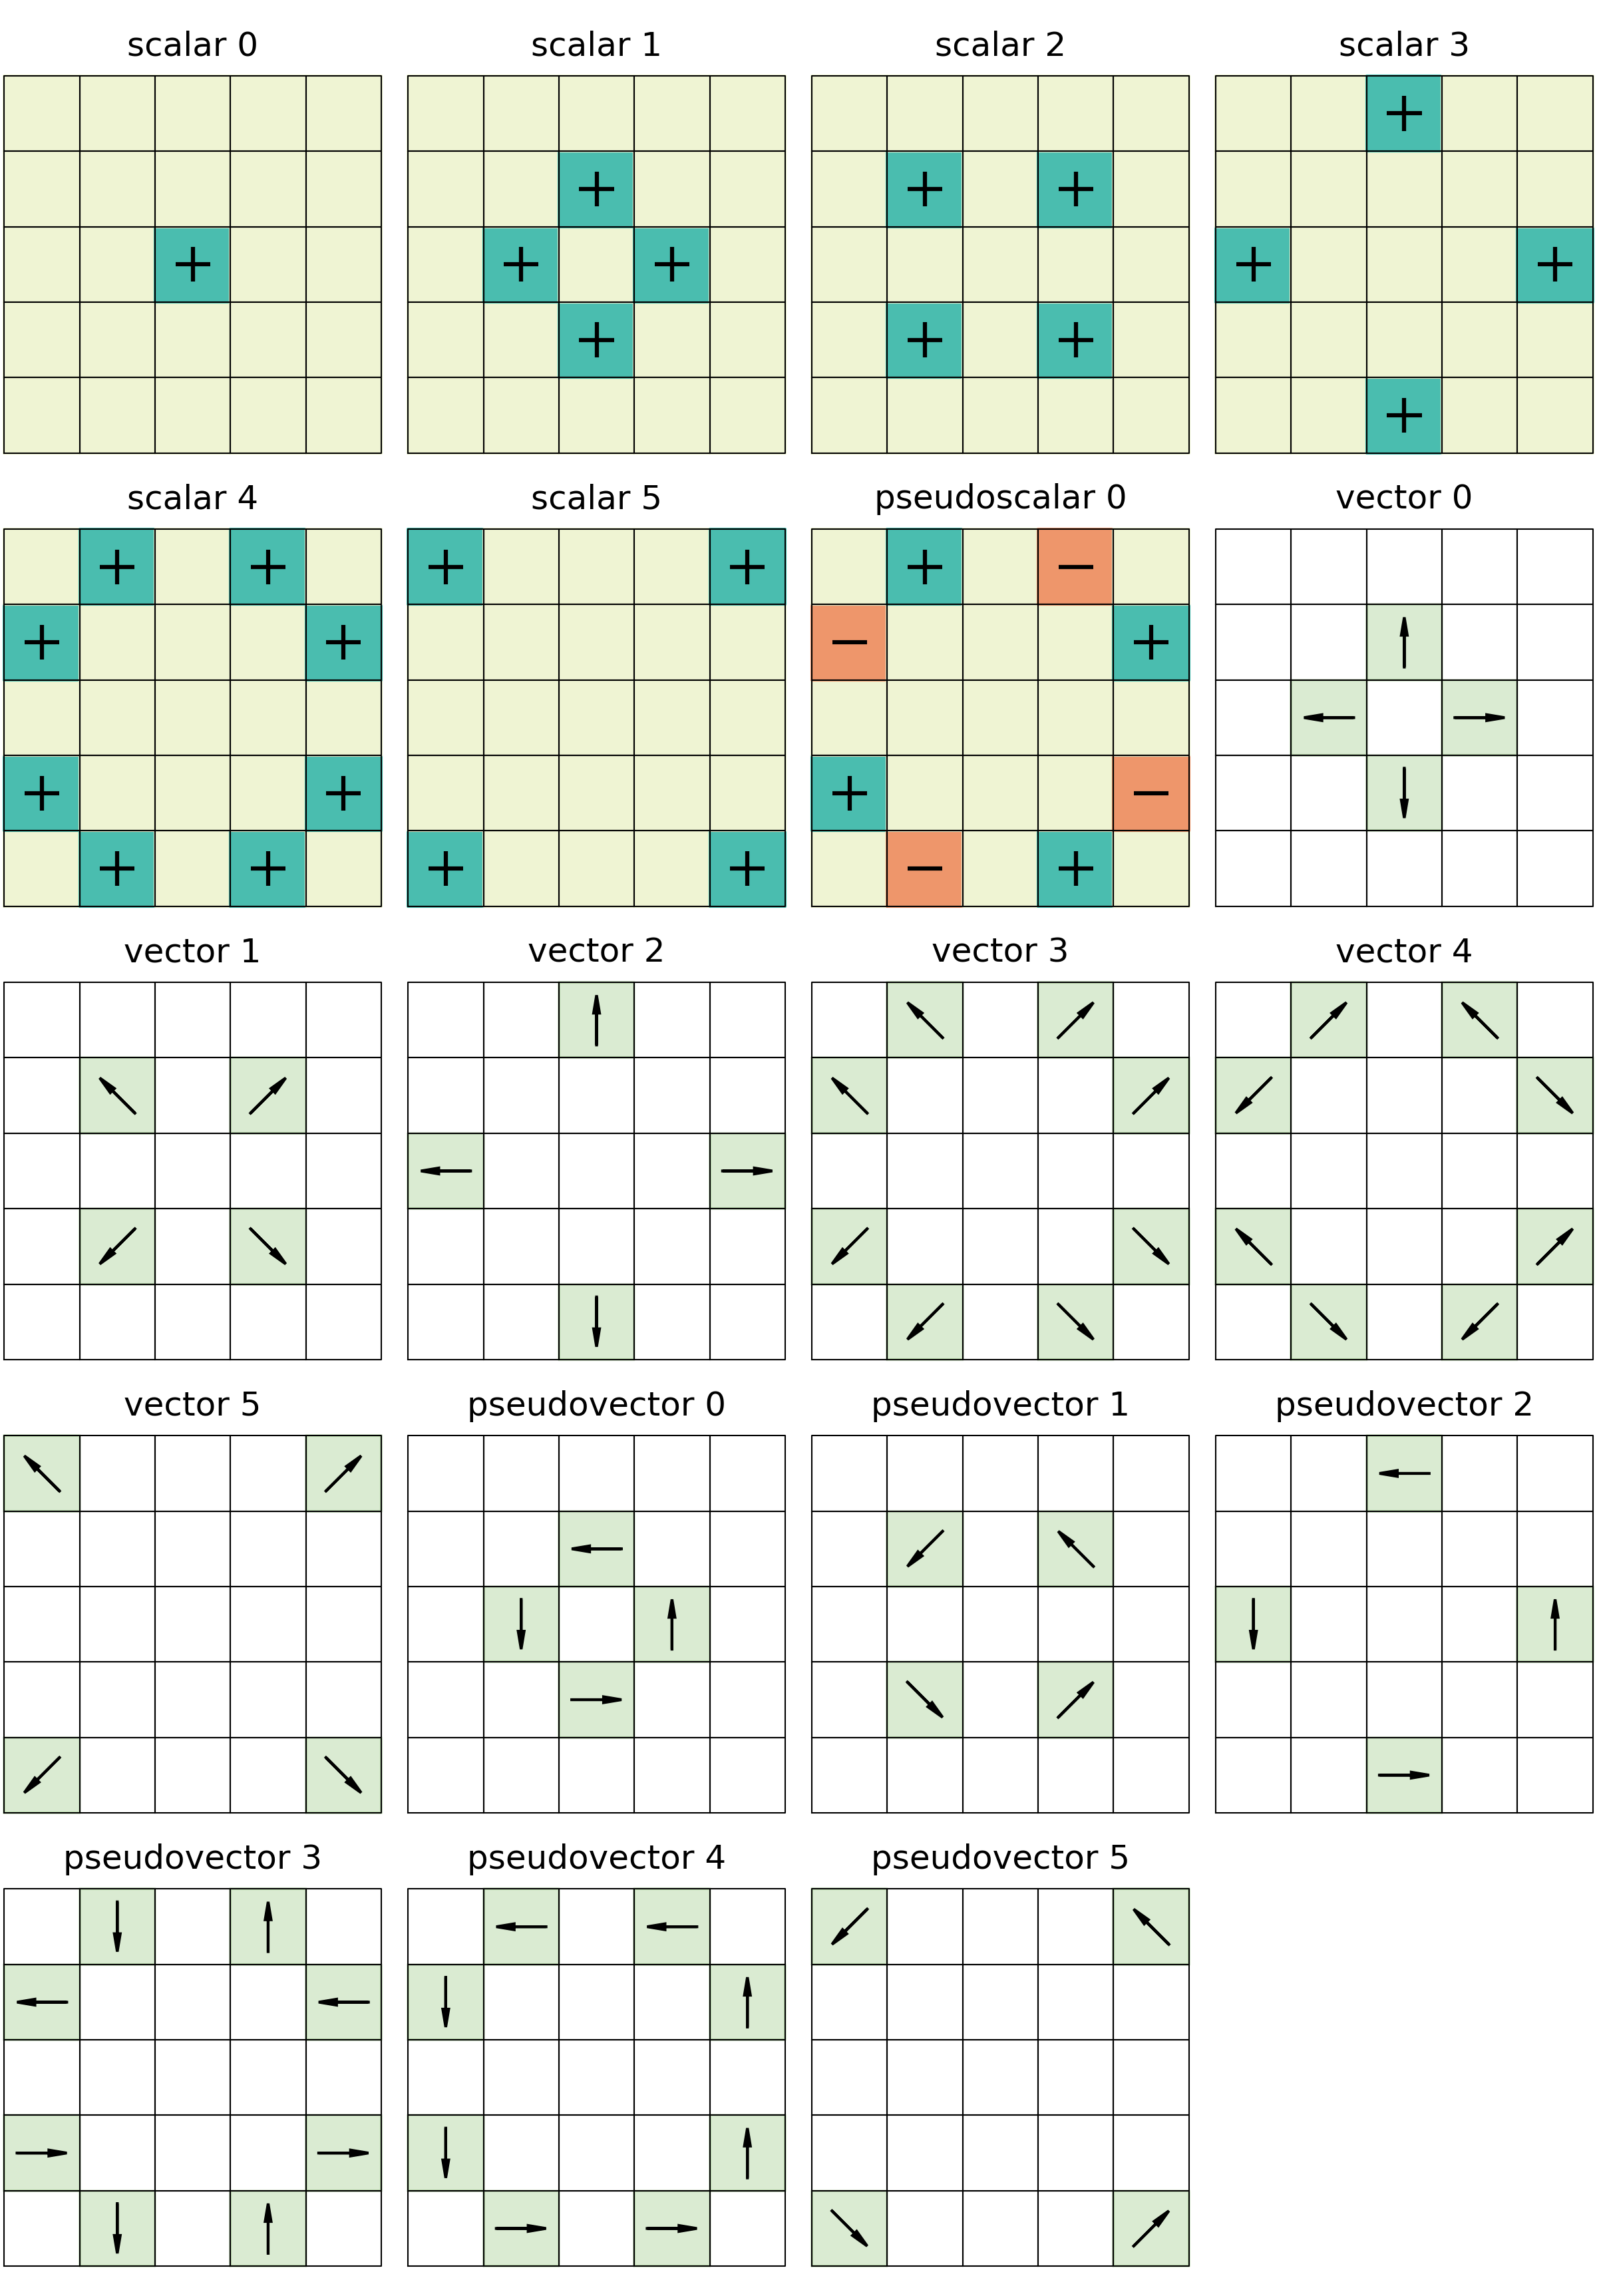
\includegraphics[width=\textwidth]{notebooks/filter_2_5.png}
  \end{center}
\caption{All the filters for $d=2$, $m=2$ ($M=5$).
Notes: Symbols and colors as in \figref{fig:filters23}.
We don't show the $2$-$p'$-tensor filters at $m=2$ because there are many of them.\label{fig:filters25}}
  \end{mdframed}
\end{figure}

\section{Expressive power of nonlinear convolution-based functions}\label{sec:universality}

Counting arguments.

Comments on locality.

We can express all linear translation equivariant functions (by just using convolutions assuming filters are same size of the image). 

We can cite that convolutions with small patches may be seen as low pass filters in some way. Reference?

\section{Implementation and numerical examples}\label{sec:examples}

How do we make the invariant filters? See \secref{sec:equivariant}.

How do we make the linear functions? See \secref{sec:convolution}.

Now show some fake-data geometric images and show the action of the $d=2$, $M=3$ filters on those images.

What do they look like? Like calculus operators! See figures.
\begin{figure}
  \begin{mdframed}
  \color{captiongray}
  \begin{center}
    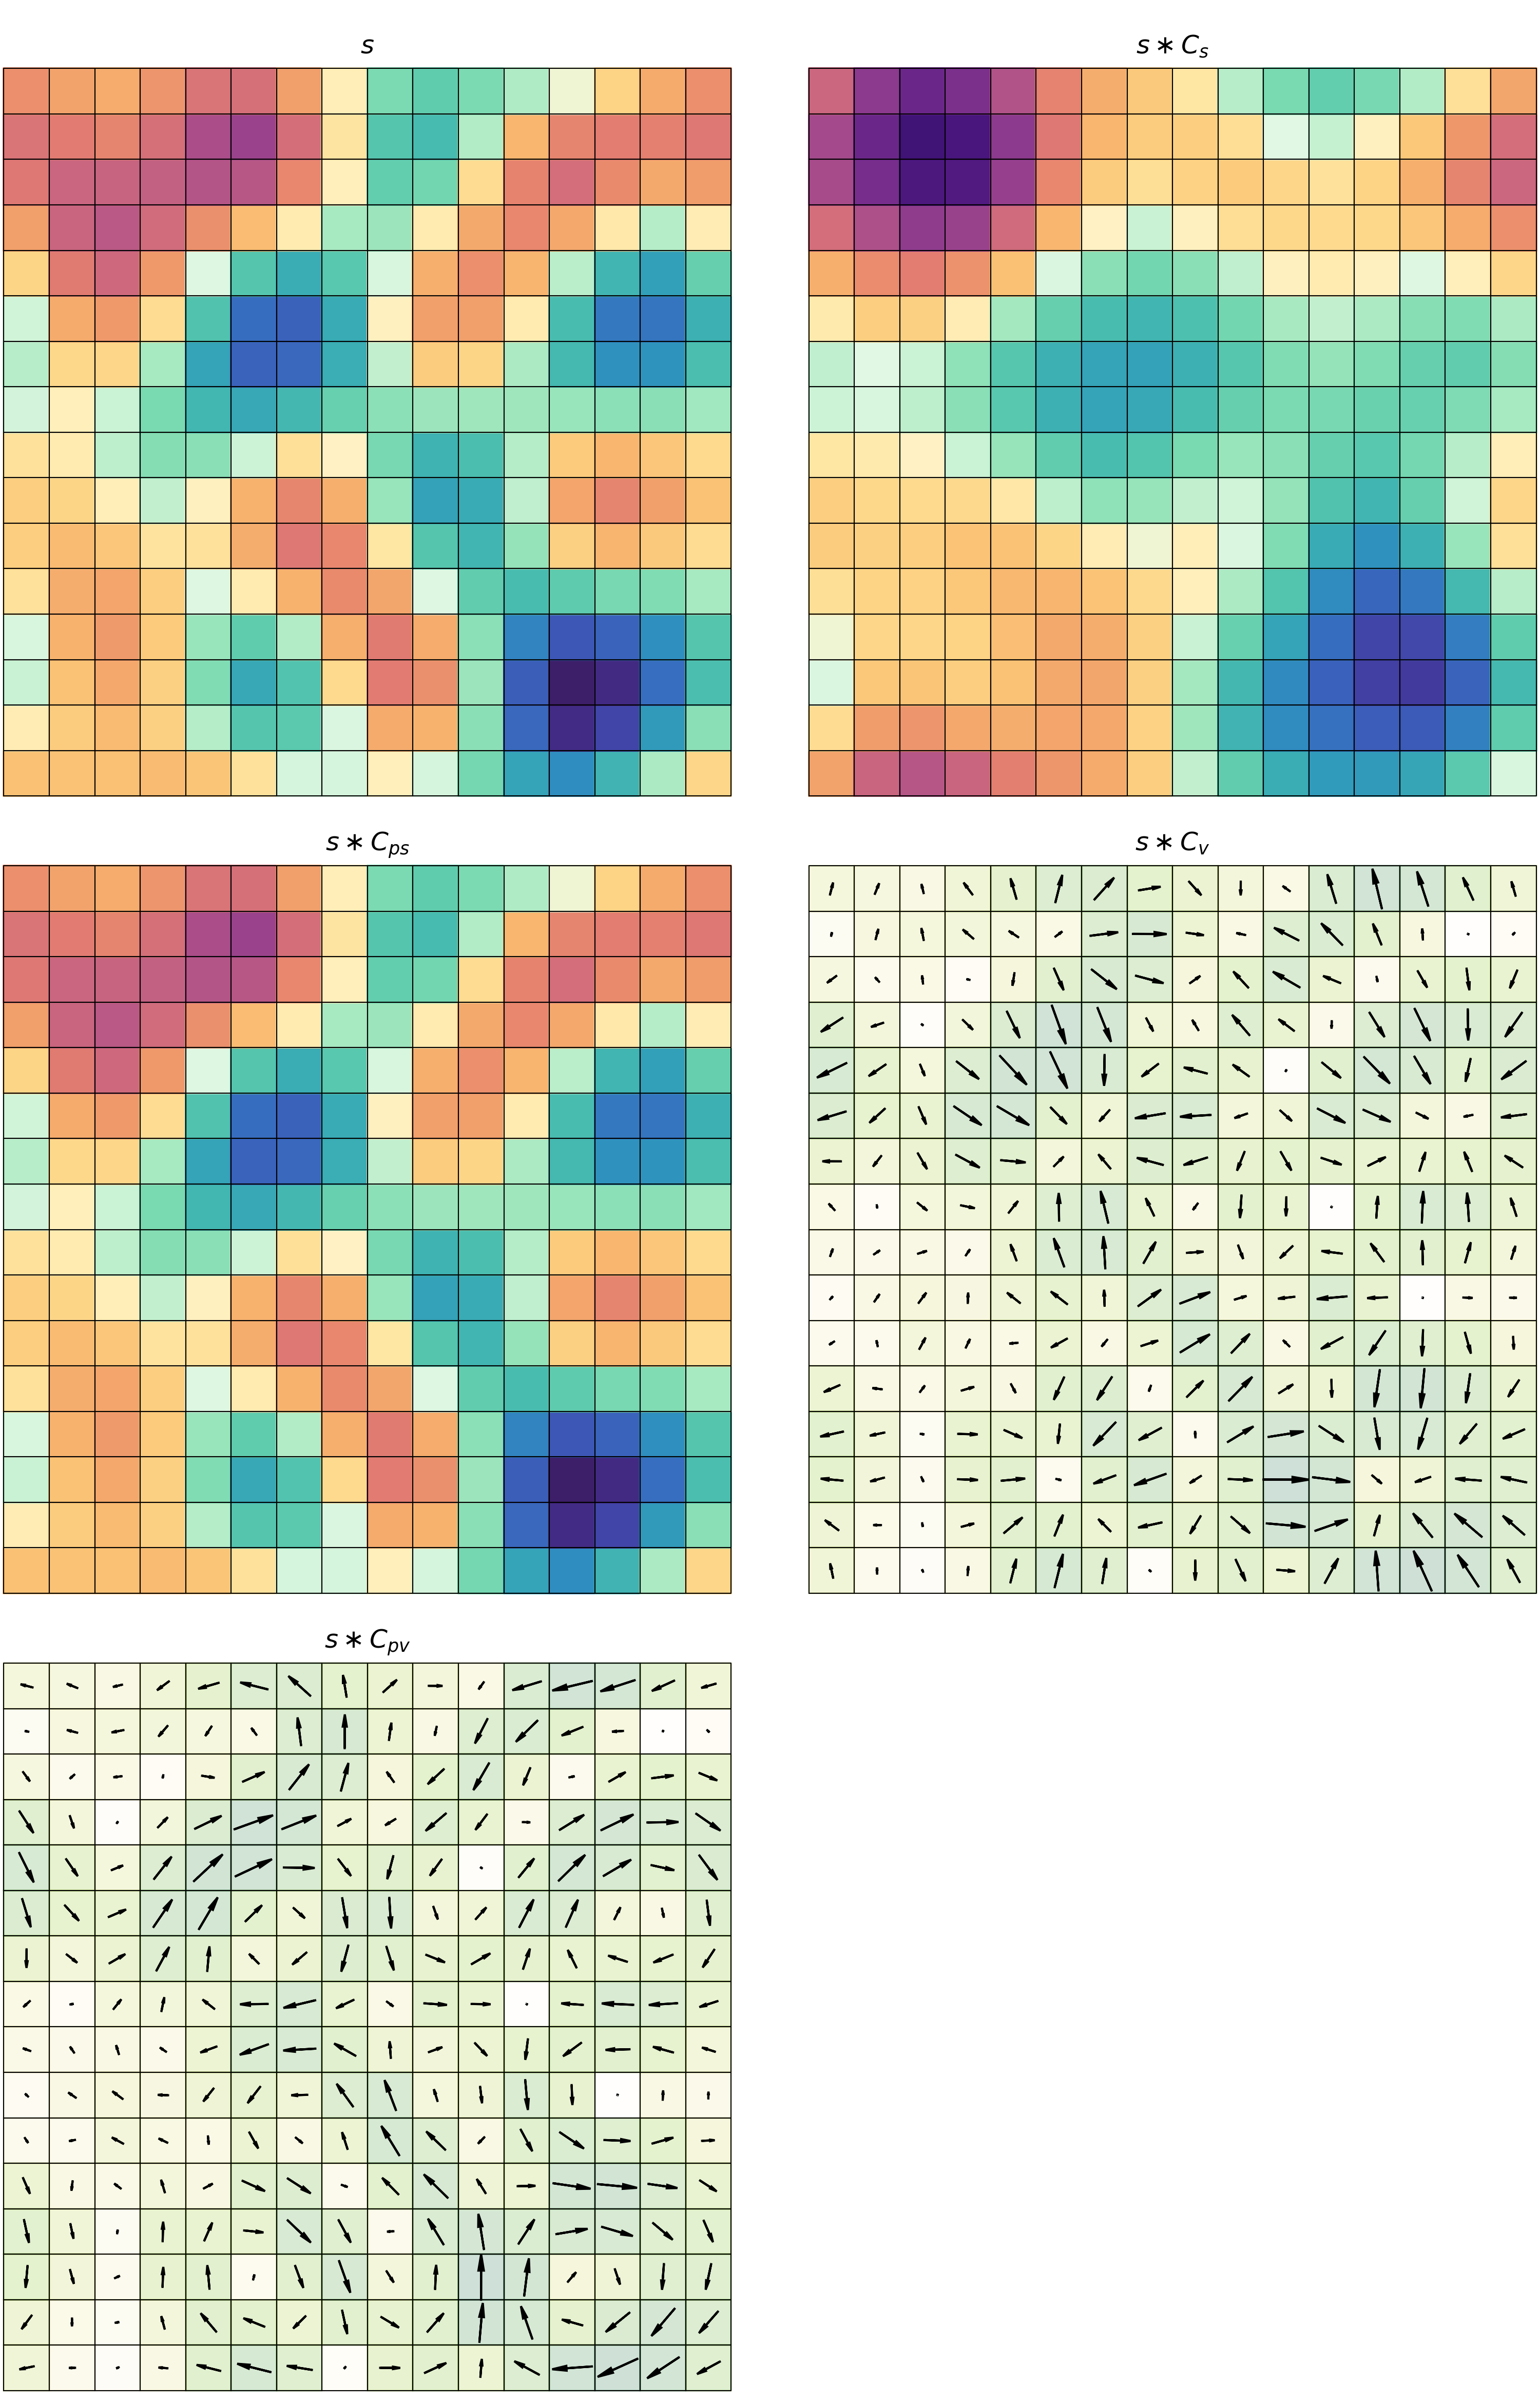
\includegraphics[width=\textwidth]{notebooks/monomials_1.png}
  \end{center}
    \caption{A scalar image $s$ and convolutions with four chosen filters.}
  \end{mdframed}
\end{figure}

Now show contractions of products of the above on those images.

\begin{figure}
  \begin{mdframed}
  \color{captiongray}
  \begin{center}
    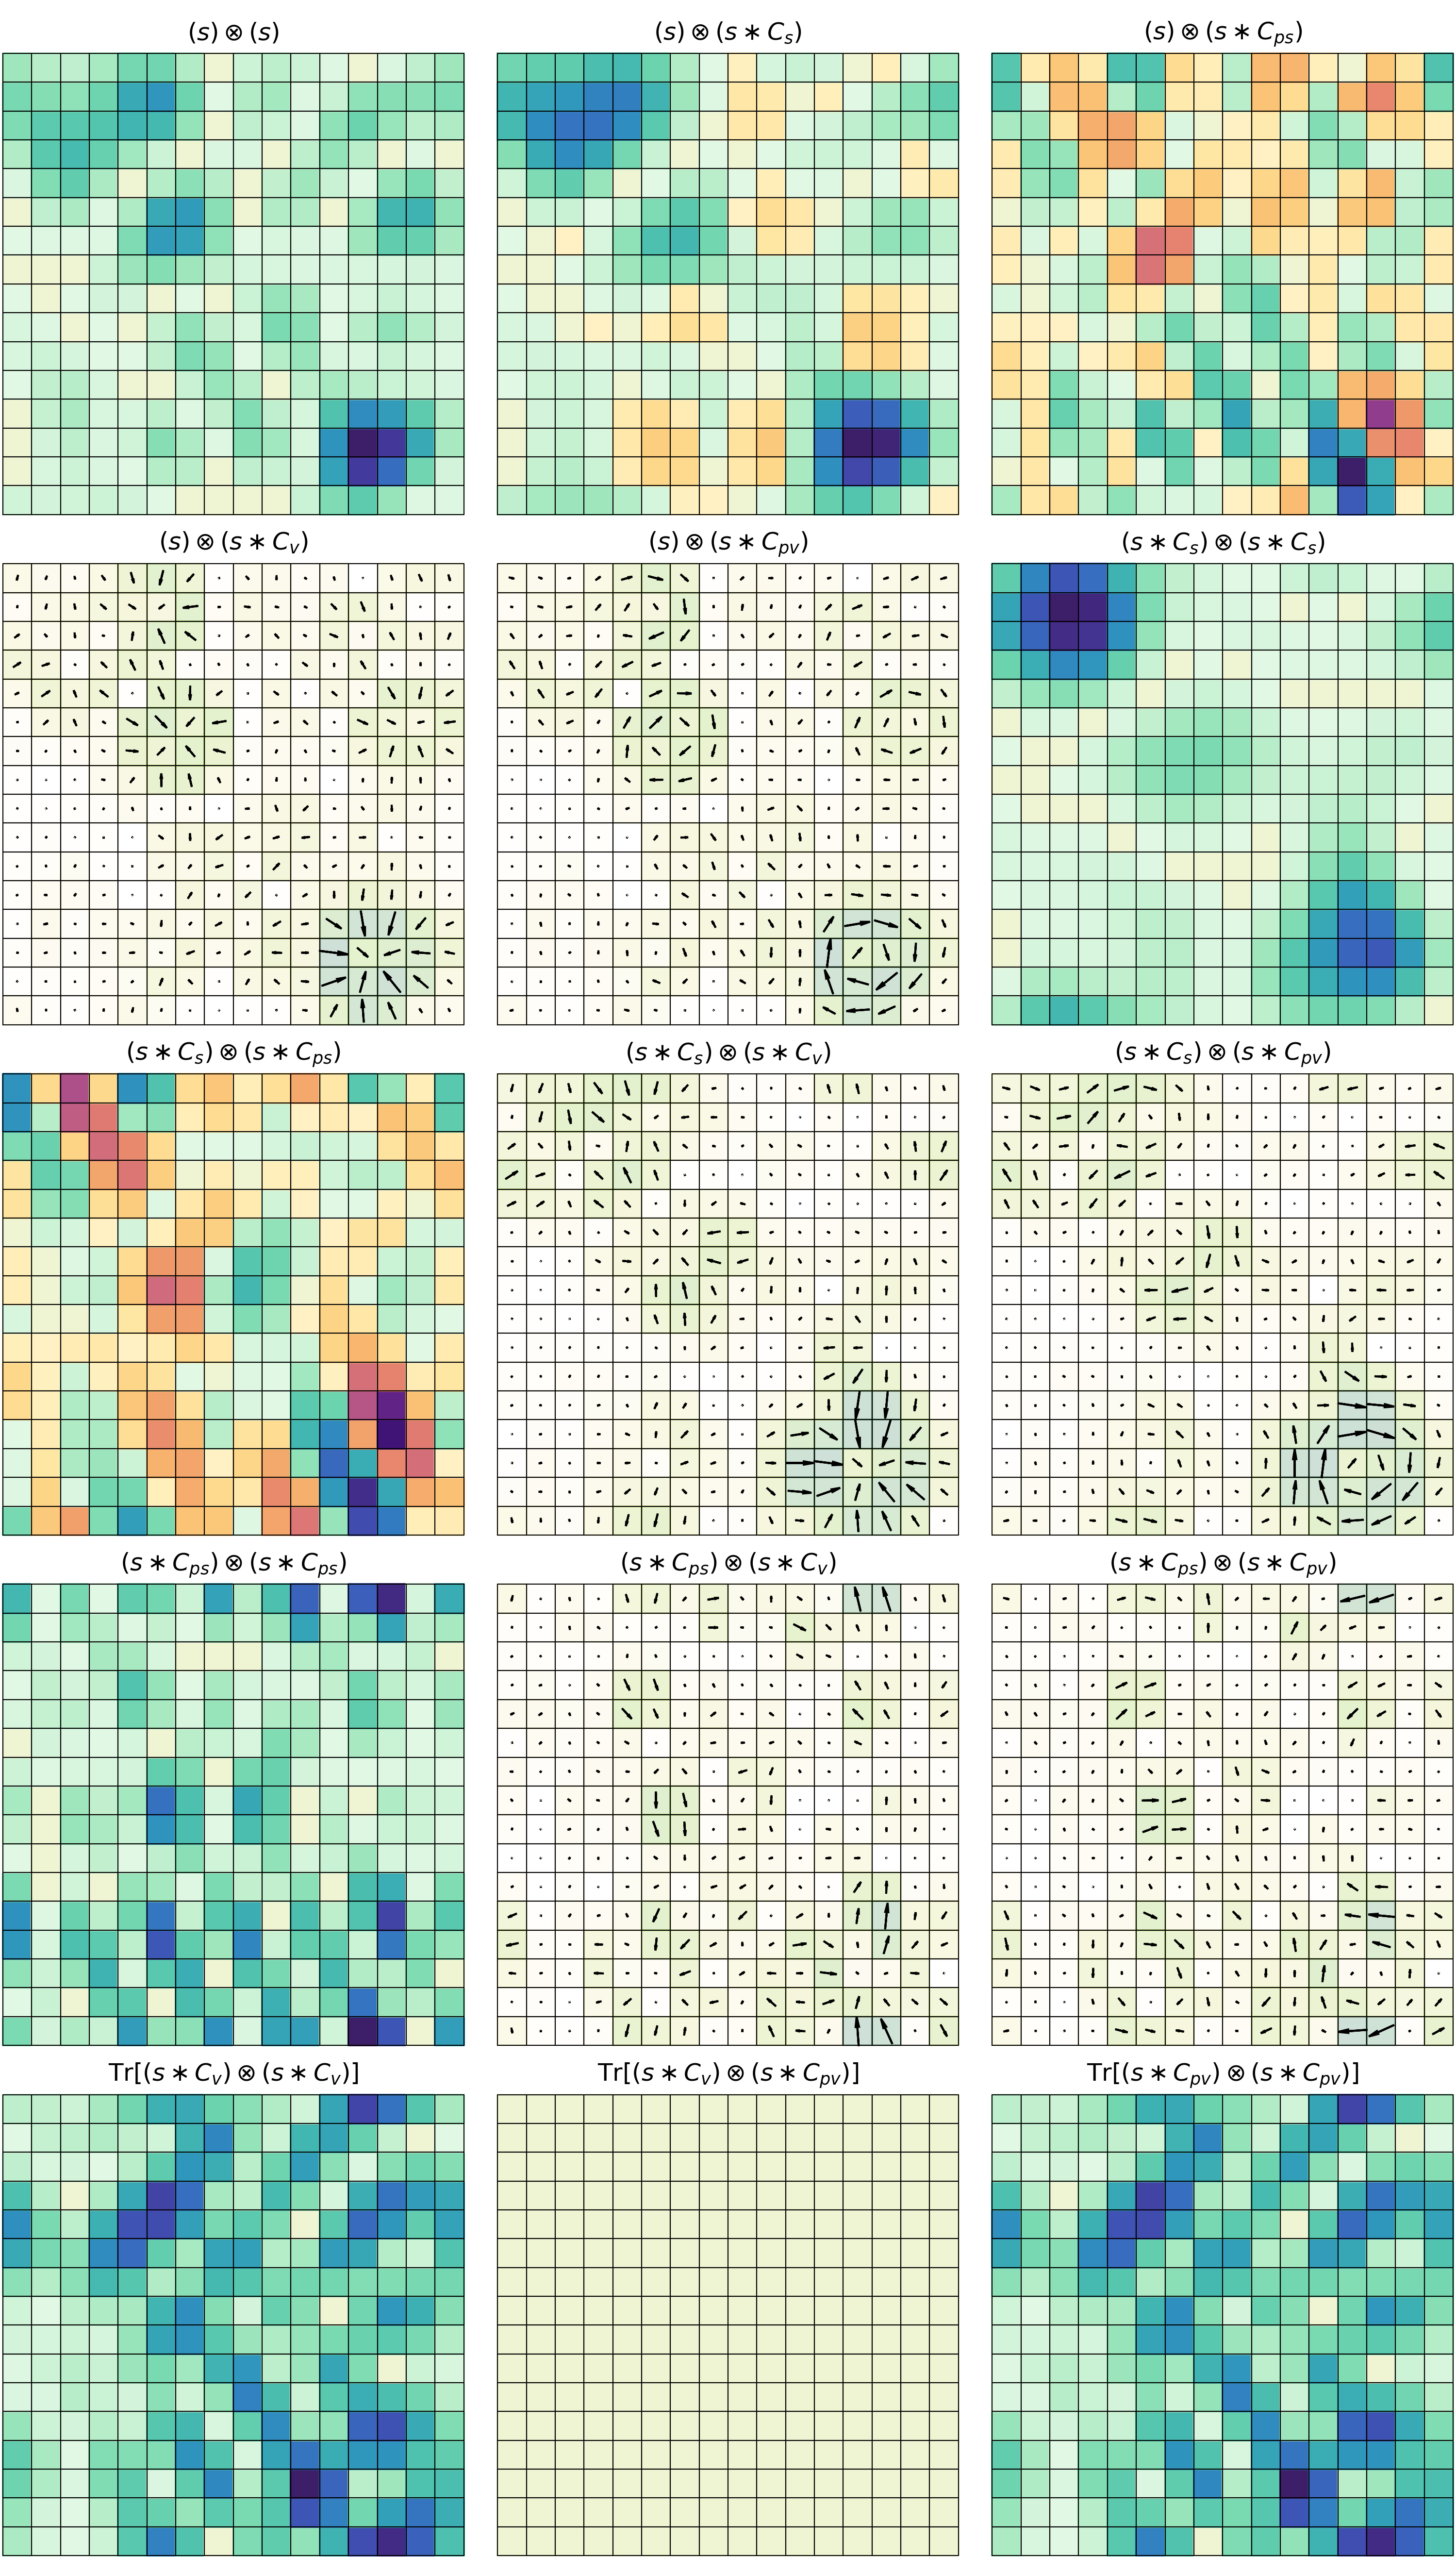
\includegraphics[width=\textwidth]{notebooks/monomials_2.png}
  \end{center}
    \caption{All unconvolved second-degree monomials of $s$, given four chosen filters. For the 2-tensor outputs (order $k=2$), we traced them back to scalars.}
  \end{mdframed}
\end{figure}


\begin{itemize}
    \item find the invariant geometric filters
    \item geometric convolution operator
    \item pixel-wise outer product
    \item contraction operator, enumeration of all contractions
    \item output index permutation, enumeration of all permutations
    \item enumeration of all monomials up to a fix order and degree 
    \item remove repeated objects (SVD or just lstsq)?
    \item linear combinations 
    \item loss function
    \item optimization
\end{itemize}


\section{Discussion}\label{sec:discussion}

Hello world

One of the strange aspects of this work is that there are two groups acting.
One is a continuous group (the Euclidean group) of translations and rotations (and reflections).
This group motivates the index summation rules and the other geometric operations in the functions we construct.
The other group is a discrete group $G_d$ appropriate for $d$-cube lattices of points; it is a sub-group of the continuous group.
This is the group we use to average the filters (to make invariant filters) and we use to define equivariance for functions of geometric images.
There are other possible image representations---other than values in pixels---that might create more continuous concepts of images.
For example, if the data are on the surface of the sphere (the sky, perhaps), it could be represented with tensor spherical harmonics, and be subject to transformations by a continuous rotation group.

But if we think in terms of a physical, generative model for imaging: Usually an image is ``taken'' of a continuous world.
That is, the kinds of geometric images we consider in this work would mainly be discretized views or samples of a larger, continuous world.
That world is subject to transformations by continuous symmetries, maybe even gauge symmetries.
It remains an open question how to think about how to use the operations and symmetries of these large, continuous groups that govern the world being viewed, when the data are only discrete, finite views of that world.

HOGG: It is interesting that the convolution operations look (in many cases) very much like discrete versions of vector calculus operations, like div, grad, curl, and so on. That's interesting, and potentially useful.

Note that we never take eigenvalues. But these are also real scalars in some cases.

Note that $k$-$1$-tensor (pseudo) filters only exist for certain triples of $(d, m, k)$.

\paragraph{Acknowlegements:}
It is a pleasure to thank Teresa Huang (JHU) and Kate Storey-Fisher (NYU) for valuable discussions.
This project made use of Python~3 \cite{python3}, numpy \cite{numpy}, matplotlib \cite{matplotlib}, and cmastro \cite{cmastro}.
All code used for making the data and figures in this paper are available at \url{https://github.com/davidwhogg/GeometricConvolutions}.

\bibliographystyle{plain}
\raggedright
\bibliography{ref}
\end{document}
